\subsection{CI/CD chains}
\label{sec:ci-cd-chains}

We use CircleCI as a continuous integration and continuous delivery platform and have configured a workflow \cite{workflow:circleci} with jobs to build, test, and deploy our service, generate a changelog, as well as build our LaTeX project. At the end of this section, there is a diagram (\autoref{fig:ci-cd-diagram}) showing our full CI/CD flow.

\subsubsection{Building, testing, and static analysis}

This part of the workflow quite simply installs the dependencies, and then builds and tests the project. Additionally, it runs the following three static code analysis jobs:
\begin{itemize}
    \item A Go linters runner: \texttt{golangci-lint}, which runs dozens of linters in parallel.
    \item A cyclomatic complexity calculator: \texttt{gocyclo}, to ensure that the code has low complexity. Otherwise, the job will exit with code 1 until we've refactored the functions in question.
    \item A developer security platform, \texttt{Snyk}, to find and fix security vulnerabilities in code, dependencies, and containers.
\end{itemize}

Besides this, we've set up SonarCloud and Better Code Hub, which provide us with more general static code analysis. For the overall results of these two and some examples of warnings, see \appendixref{appendix:static-code-analysis-results}.

\subsubsection{Deploying our service}

CircleCI will also:
\begin{itemize}
    \item Publish a GitHub release when merging to the master branch
    \item Push our changes to the four images in Docker Hub (the server, frontend, Prometheus, and Grafana)
    \item Deploy by performing a rolling update to the aforementioned services in Kubernetes
    \item Apply infrastructure changes via Terraform
\end{itemize}


\subsubsection{Generating a changelog, and building the LaTeX project}

We use CircleCI Github Changelog Generator \cite{tool:changelog-generator} to generate a changelog based on our tags, issues, labels and pull requests on GitHub.

To include a build of the LaTeX project in the CircleCI workflow, we've written a script to let CircleCI run a custom Docker image, build a PDF, and then commit it to the branch.

\begin{figure}[H]
    \makebox[\textwidth][c]{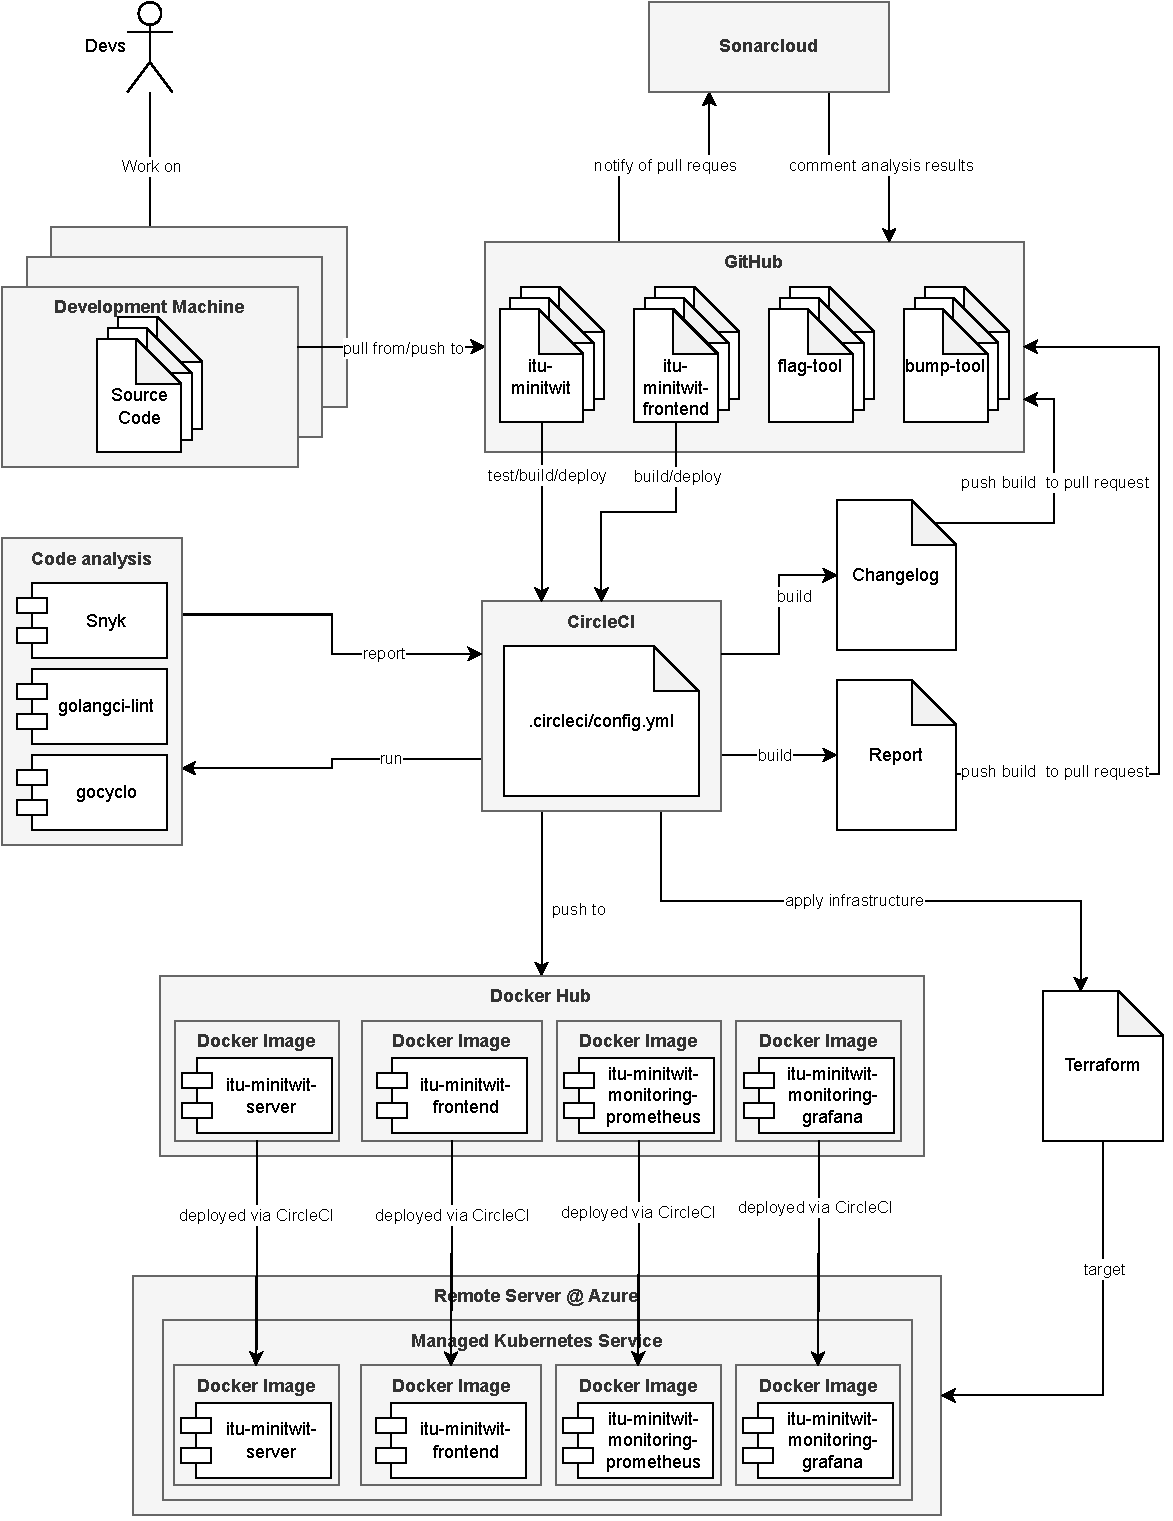
\includegraphics[width=0.85\paperwidth]{workflow/ci-cd-workflow.pdf}}
    \caption{A diagram showing our CI/CD flow.}
    \label{fig:ci-cd-diagram}
\end{figure}
